\documentclass[8pt,a4paper]{report}
\usepackage{hyperref}
\usepackage[latin1]{inputenc}
\usepackage{xcolor}
\usepackage{textcomp}
\usepackage{amsmath}
\usepackage{amsfonts}
\usepackage{listings}
\usepackage{amssymb}
\usepackage{hyperref}
\usepackage[T1]{fontenc}
\usepackage[scaled]{beramono}
\newcommand\Small{\fontsize{9}{9.2}\selectfont}
\newcommand*\LSTfont{\Small\ttfamily\SetTracking{encoding=*}{-60}\lsstyle}
\usepackage{url}
  \lstset{basicstyle=\ttfamily\tiny\color{blue}}
\usepackage{graphicx}
\usepackage[]{algorithm2e}

\title{Project Report\\\textsc{DEVS Ex Machina}}
\author{Ben Cardoen\\Pieter Lauwers\\Stijn Manhaeve\\Tim Tuijn\\Matthijs Van Os}
\date{}
\begin{document}
\maketitle
\tableofcontents{}

%
\chapter{Summary}
%
\section*{}
The project implements a C++ port of the PyPDEVS project, extended with conservative synchronization and a change in system architecture from distributed simulation on several nodes (asymmetric mp) to a symmetric multiprocessing architecture. \\The summarized goal of the project is to provide an implementation of the offered DEVS formalisms with significantly lower execution time by levering the smp architecture.

\section*{Terminology}
The literature sometimes exchanges terms, to avoid any confusion the following frequent terms are listed with their associated meaning as used in this document:
\begin{itemize}
  \item Core : alias kernel. Single instance, containing a set of models it is responsible for, exchanges messages generated by those models and keeps time state. Can correspond with Logical Process in terms of what it represents.
  \item Logical Process : set of models with strong internal coherence.
  \item Distributed parallelism : computation distributed over several physically separated machines communicating by means of a network stack.
  \item SMP : symmetric multiprocessing, running a parallel computation on several distinct CPU cores/threads on the same machine with shared memory (and/or cache).
  \item message : any exchange of high level information between entities, user defined or for inter-kernel synchronization.
\end{itemize}

\chapter{Planning}
\section{Parallel}
\begin {itemize}
\item GVT integration : week 0-1, Ben and Tim
\item Conservative : week 2-3 , Ben and Tim
\end {itemize}
\section{General}
\begin {itemize}
\item Dynamic Structured : week 1-3 Stijn
\item DevStone and examples : week 0-2 Matthijs and Pieter
\item Serialization : week 0 Pieter
\item Simulation control : week 1-3 Matthijs and Pieter  
\item Tracers : week 0 Stijn
\item Benchmarking PyPDevs Adevs : week 3 Matthijs and Pieter
\end {itemize}
\section{Optimization}
Week 4 , general review.

\chapter{Architecture Analysis}
\section{Implementation language}
Python is a very powerful language, but due to its interpreted nature it suffers from a performance point of view. Python's GIL \cite{gil} makes this issue even more serious whenever multi-threading is required. Although it relieves the developer from tracking resource allocation, this comes at a price in the overhead caused by the GC. \\
In contrast, C++ offers low-level powerful thread primitives, but requires the developer to have a very deep understanding of parallel programming techniques. By using RAII, a C++ developer can leverage safe resource (de)allocation without losing performance.\\
A significant advantage Python offers a developer is relative cross-platform capability. This is non-trivial for a C++ developer, since at the very least the toolchains will be radically different in usage, and sometimes even in implementation of the C++ standard. The edit-build-test cycle is also non-trivial for a large C++ application, whereas in Python this is negligible. In contrast, Python does not offer the programmer any of the C++ compiler's many compile time checks (static typechecks and program analysis).

\section{Operating system support}
The project requires a compliant C++11 compiler and library, but beyond that is not really bound to special features. For testing, GTest is a requirement, and the only two other dependencies are the ubiquitous Boost and Cereal, the last is provided with the project as it is header only.

\section{Object representation}
In Python everything is a reference, and since the DEVS formalisms require that the user be allowed to override most of the basic entities, the best representation for an object was a shared\textunderscore ptr. Passing by value could have been safer (e.g. between threads) but would introduce slicing.\\ Another advantage was that we would use as little memory as possible, for example sending a message means passing an const reference to a shared pointer, which is usually equal in size to 2 pointers. By passing by const ref we minimize most of the penalty usually involved in copyconstructing shared pointers. \\
The only downside is the synchronized access to the reference count in the shared pointer. There is also a need for more boilerplate code to use shared pointers in containers (providing pass-through hash function, comparison etc). 

\chapter{Design}
\section{Overview}
We've slightly departed from the PyPDEVS structure, to allow for more encapsulation and decoupling of the core entities. This clear separation of data and responsibilities between classes made the threading part of the project easier (no or minimal shared state). See the \hyperref[simpledesign]{Simple Design figure \ref*{simpledesign}}.\\

\begin{figure}[h!]
	\makebox[\textwidth][c]{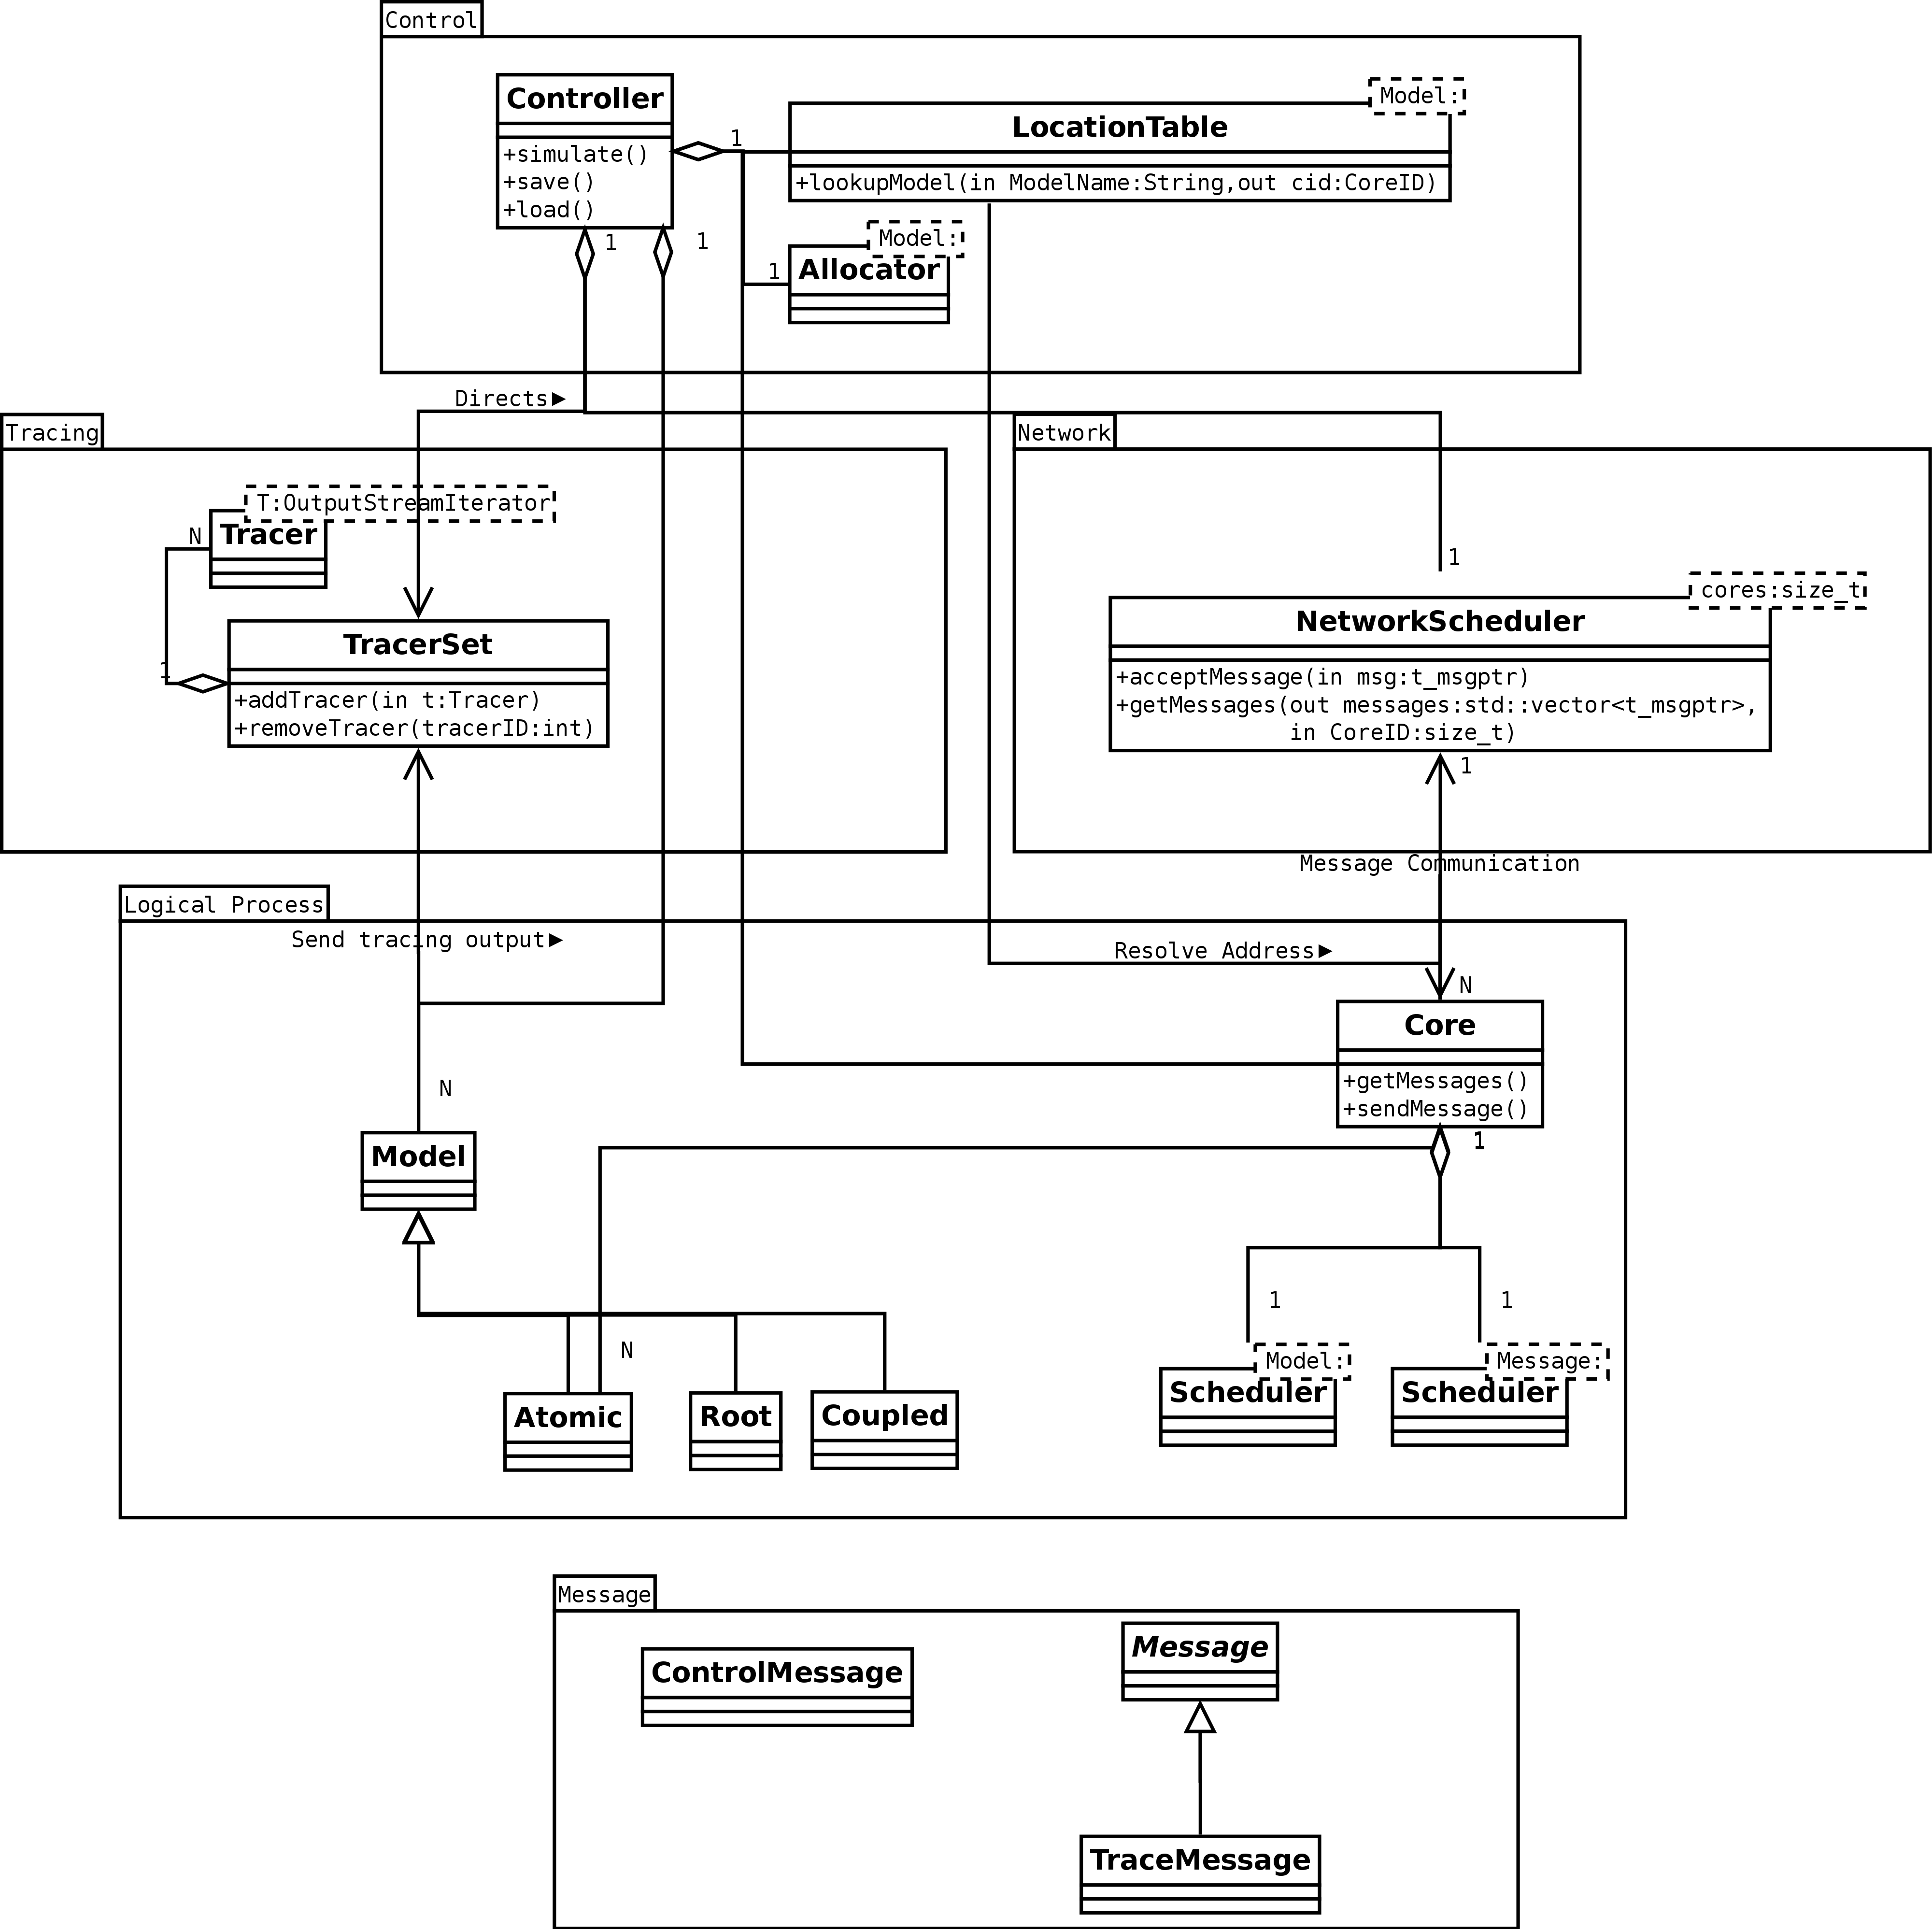
\includegraphics[width=1.5\textwidth]{Design.png}}
	\caption{Simple Design}
	\label{simpledesign}
\end{figure}

\section{Translating Dynamic Typing to Static Typing}
To represent objects that can be at runtime any type chosen by the user, we had 2 options : void* which is highly fragile in use, and impossible to serialize, or std::string(), which can double as an "anytype" by storing a serialized object inside the string, should this be required. \\This leaves the same degree of freedom dynamic typing grants to the user in PyPDEVS, with the added benefit of some checking provided by the compiler. Consider for example a user who stores an object serialized into the payload string of a message object, the compiler can in advance detect if the serializing object is at least serializable. \\ Misuse would either surface during compilation, or at worst could be checked with casting or exceptions. Misuse of void* could result in anything from undefined behaviour to stack corruption.

\section{Class decomposition}
The active entities in the project were discovered using several methods: use cases, argumentation and counterargumentation during the weekly meetings, and studying the existing implementation. This led to the following simplified decomposition:
\begin{enumerate}
\item Model : provides DEVS formalism implementation of an Coupled/Atomic model.
\item Core : drives transitions, exchanges messages, synchronizes
\item Controller : Constructs simulator, controls simulation
\item Tracer : Traces output
\end{enumerate}
The other classes bind/create instances of the above (e.g. LocationTable, Allocator, Factory), or provide essential functionality (e.g. Message, Network, Scheduler)\\
For a full overview, please consult the documentation generated by doxygen.

\section{Network -- Kernel communication}
PyPDEVS uses MPI to exchange messages between kernels, whereas we could use shared memory to communicate between kernels (each running on 1 or more threads). We created a network architecture mimicking the approach used by PyPDEVS, without sacrificing the speed and ordering advantages of shared memory. The Network class consists of a single locked receiving port, and has for each existing kernel an outgoing queue. Receiving a message locks the network for the time it needs to place it on an integer indexed queue (very fast). If a kernel wants to receive messages it can do so if/when it is ready to do so, this only locks if at the same time a message is being received by the network.\\ Several kernels can pull messages without contention in parallel from the network (since the output queues are not shared). \\This is illustrated in \hyperref[networkdesign]{Network design figure \ref*{networkdesign}}.

\begin{figure}[h!]
	\makebox[\textwidth][c]{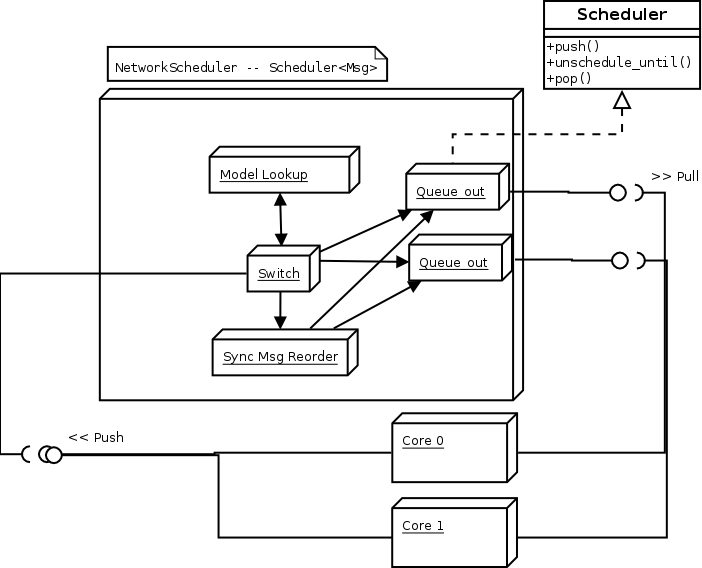
\includegraphics[width=\textwidth]{network.png}}
	\caption{Network cooperation diagram}
	\label{networkdesign}
\end{figure} 
Early benchmarks showed a repeatable throughput of 5e5 msg/s, with 4 kernels on modest hardware. The problems of (unintentional) out of order receipt and potential loss of messages are a non-issue in this context, since we use FIFO queues and loss of a message would implicate severe system failure (in which case message loss is the lesser problem).\\
Another advantage of hiding the message exchange behind a shared Network class instance is that, should this be required in the future, the kernel could run on different machines without requiring much redesigning of the system. An RPC implementation would simply have to implement the Network class on both sides.

\section{Tracing}
The tracing uses template programming, and is largely asynchronous w.r.t. the simulator kernels. This can be seen by the high utilization values when benchmarking the examples.
The tracing component makes heavy use of template programming. For more detailed information, please refer to \href{run:./tracersReport.pdf}{tracersReport.pdf}.

\section{Models}
The models hide all implementation details for the particular DEVS formalisms, without limiting the user to extend into any subclassed model of his/her choice. The use can focus on what he/she wants the model to emulate, and not worry about for example locking, allocation etc. We refer to the manual for more information about the creation of these models.

\section{Scheduler}
The scheduler from the prototypes was reused, with little to no changes (barring a few bugfixes). An unsynchronized version was implemented for comparison purposes.

\section{Controller}
For the controller, care was taken in making the interface both functional and minimal. The default configuration is quick to set up, and customization is possible should the user require it.

\section{Serialization}
For serialization we used the Cereal \cite{cereal} header-only framework. We have used separate load and save functions for full flexibility. For each type that occurs in the form of a pointer we implemented a static load and construct function since the object first has to be created before the saved data can be imported. Cereal has a small coupling with the code (models) that has to be written by the user as the user has to register his own classes due to polymorphism.

\chapter{Non-functional requirements}
\section{Correctness}
\subsubsection{Testing}
The use of the jenkins CI was heavily leveraged, in combination with extensive testing. Any feauture increment could only be merged into the project if it passed the developer's own jenkins instance.
\subsubsection{Thread races and deadlock}
Deadlocks and race conditions are very hard to debug, let alone prevent. To help us in this area as much as possible we used prototypes of threaded code in the tests before merging them into the main classes, and each build is checked with ThreadSanitizer \cite{tsan} which proved invaluable in preventing races and deadlocks in the threaded codepaths.
\subsubsection{Memory leaks and undefined behaviour}
With most entities represented as smart pointer, the need to ensure a leak free simulator nevertheless remained. To check for allocation misuse and a whole other series of errors we used Valgrind \cite{vg}. This meant for example that we detected a leak caused by circular referencing smart pointers.

\subsubsection{Teamwork}
We met at least once every week (barring the exam period), with each meeting having a formal report. Whenever required, teammembers used video conferencing to solve critical bugs or discuss design/coding issues.
\subsubsection{Code review}
Although there was no real formal code review done up to now, we've had several debug sessions reviewing each others code. This means the most critical used sections of the code are allready reasonably well reviewed, albeit not formally.
\subsubsection{Portability}
We develop on Unix, Windows and MacOSX.

In Windows we chose the Cygwin platform instead of MinGW to compile our project on. This because we make use of the C++11 std::thread objects; MinGW doesn't support POSIX threads. When building the project with GTest on Windows you need to use the -std=gnu++11 flag instead of the standard -std=c++11 flag, because we need the GNU extensions to correctly link everything.

\chapter{Functional requirements}
\section{DEVS Formalisms}
\section{Single core}
The single core implementations follow exactly the runtime behaviour shown by the PyPDEVS simulator. We've chosen to emulate the Select() function with an integer priority value the user can set. This saves 1 virtual function call per transition and can quite easily be optimized by the compiler since it remains constant.
\subsection{DirectConnect}
The directConnect algorithm has gone relatively unchanged from its implementation in PyPDEVS, though the role of the RootDEVS class has been simplified somewhat. Its main function has been reduced to executing directConnect and then storing the resulting list of connected atomic models.
\subsection{Dynamic Structured}
Only the removal/addition of connections is currently supported. Unlike the PyPDEVS, we will try to keep a removed model intact when it is removed from the simulation.
\subsection{Parallel}
\subsubsection{Optimistic}
Optimistic time synchronization requires an implementation of timewarp, and more extensive locking than would be required for conservative. The GVT algorithm (Mattern \cite{Mattern}) runs on a separate thread from the simulation kernel threads, so care must be taken that they don't deadlock, but don't race either.
\subsubsection{Conservative}
Conservative time synchronization is still under development.


\chapter{Obstacles}
\section{Virtualization}
Virtualization proved a significant hurdle by exposing potential faults. Standard compliant code was found to be leaking memory by not calling container member destructors but only on a VM with Linux as Guest and Windows as Host. This was never reproducible in another setting.
\section{Threading}
libstdc++'s std::string implementation appears to be still Copy On Write (despite 21.4.1 p6 from the C++ standard) \cite{cpp}, triggering an alert by threadsanitizer for a possible race whenever a string was supposedly copied but internally still stored as a reference to the same object. Explicitly invoking the string constructor with the char[] proved to be a safe workaround here. Note that this problem is a known issue \cite{cow}.
\section{Toolchains}
To develop we used the required toolchains:\\ g++/clang++ as compiler, Eclipse+CDT as IDE, git for dvcs, jenkins as ci, cmake as build tool supplemented with some shell and python scripting.
\section{Logger}
The recommended logger (g3log), while powerful and fast, proved a dead end since it does not compile on Cygwin. 
Stijn therefore wrote his own implementation.\\
This implementation only covers the most basic needs:
\begin{itemize}
	\item asynchronous output
	\item thread safe
	\item multiple logging levels currently, the following 4 levels are supported:\\
		\emph{INFO}, \emph{DEBUG}, \emph{WARNING} and \emph{ERROR}
	\item levels can be individually switched on/off at compile time
	\item No logging code is executed whatsoever if the logger is disabled
	\item log messages contain filename and line number of the log command
\end{itemize}
It therefore lacks certain key features such as
\begin{itemize}
	\item crash safe
	\item custom assert that will log an error before shutting down
\end{itemize}
Chances are that we will wait with implementing these features until we actually need them.
\chapter{Performance Analysis}
Whenever we made big design/architecture decisions, we first wrote some prototyping testcode to prove the viability (e.g. Network, Tracing, Logger).
\section{First comparison}
We use perf to get statistically sound benchmarks. The command run was :
\lstinline!$perf stat -r {rounds} {command}!\\

\subsection{Classic}
An endtime of 3.6e6 was set, and both examples run against each other.
\lstinputlisting[]{pycla.txt}
The following shows a recording of the C++ implementation of the same example.\\
\lstinputlisting[]{cpcla.txt}
\subsubsection{Conclusion}
The C++ port is approximately 12.906 times faster.

\subsection{Dynamic structured}
An end-time of 3.6e6 was set, and both examples run against each other.
\lstinputlisting[]{pydyn.txt}
The following shows a recording of the C++ implementation of the same example.\\
\lstinputlisting[]{cpdyn.txt}
\subsubsection{Conclusion}
This result is still warped due to the startup/shutdown time of GTEST, but allready the C++ port is roughly 7.05 times faster, only page faults and migrations are worse (but being worked on).
\subsection{Parallel}
With GVT not yet active, an endtime of 3.6e6 was used (as before).\lstinputlisting[]{pypar.txt}\
The following shows a recording of the C++ implementation of the same example.\\
\lstinputlisting[]{cppar.txt}
\subsubsection{Conclusion}
The C++ port is approximately 19.6 times faster.

\section{Logger}
We have also conducted a small benchmark to compare the raw power of our logger and the proposed g3log.
We let each logger print several hundred thousand messages to a file. These are the performance statistics:
\subsubsection{g3log}
\lstinputlisting[]{g3log.perf}
\subsubsection{Our own logger}
\lstinputlisting[]{own.perf}
\subsubsection{Conclusion}
While the difference is considerable, we should keep in mind that g3log generates timestamps for each message. It also contains several features that our logger doesn't, such as crash safety. Moreover, g3log allows the user to dynamically change which log levels are filtered, while this can only be decided at compile time for our logger. This can be clearly seen in the amount of branches.

\section{Further work.}
Further optimizations included but are not limited to: 
\begin{enumerate}
\item Custom memory allocators/pools (boost, ...)
\item Profiling guided recompilation
\item Detecting bottlenecks with perf and gprof.
\item ...
\end{enumerate}

\begin{thebibliography}{1}


  \bibitem{cow} \url{https://gcc.gnu.org/bugzilla/show_bug.cgi?id=21334#c47}

  \bibitem{Mattern} \url{http://citeseerx.ist.psu.edu/viewdoc/summary?doi=10.1.1.111.2811}
  
  \bibitem{gil} \url{https://wiki.python.org/moin/GlobalInterpreterLock}
  
  \bibitem{tsan} \url{https://code.google.com/p/thread-sanitizer/}
  
  \bibitem{vg} \url{http://valgrind.org/}
  
  \bibitem{perf} \url{https://perf.wiki.kernel.org/index.php/Main_Page}
  
  \bibitem{cereal} \url{https://uscilab.github.io/cereal/}
  
  \bibitem{cpp} \url{http://www.open-std.org/jtc1/sc22/wg21/docs/papers/2014/n4296.pdf}

  \end{thebibliography}
\end{document}
